\documentclass[11pt]{article}

\usepackage{filecontents}
\usepackage{graphicx}
\graphicspath{{/Users/laci/Schule/Diplomarbeit_GitHub/LATEX_DOKU_DA/src}}
\usepackage{tabularx}
\usepackage{multirow}
\usepackage{xcolor}
\usepackage{caption}
\usepackage[autostyle]{csquotes}
\usepackage{circuitikz}
\usepackage{amsmath}
\usepackage{textgreek}
\usepackage{siunitx}
\usepackage[utf8]{inputenc}
\usepackage[ngerman]{babel}
\usepackage[margin=2.5cm]{geometry}
\usepackage[none]{hyphenat}
%==========================================================================
\usepackage{fancyhdr}
\pagestyle{fancy}
\fancyhead[L]{\MakeUppercase{Diplomarbeit 5BHEL 23/24}}
%\fancyhead[R]{\chead{
\includegraphics[width=\textwidth]{src/TGM.jpg}}}
\fancyfoot[L]{\small{Al-Maytah, Schweitzer, Szabo}}
\fancyfoot[C]{}
\fancyfoot[R]{\arabic{page}}

\usepackage[round, sort, authoryear]{natbib}
%\usepackage[nottoc]{tocbibind}
%==========================================================================
%==DOKUMENTBEGINN==========================================================

\begin{document}

%==========================================================================
%==TITELSEITE==============================================================

\begin{titlepage}
	
	\title{\textbf{\Huge{Diplomarbeit}}}
	\maketitle
	\thispagestyle{empty}

	\begin{center}

		\hfill \break
		\hfill \break
		\hfill \break
		\textbf{\Large{Gesamtprojekt}} \break
		\par
		\textbf{\LARGE{RoboGlove - Bionische Hand}}

		\hfill \break
		\hfill \break
		\hfill \break
		\hfill \break
		\hfill \break

		\begin{tabular}{p{10cm}p{1cm}l}
			3D-Druck, Mechanik und User-Interface-Programmierung \\
		\end{tabular}

		\begin{tabular}{p{3cm}p{2cm}l}
			Amir Al-Maytah & 5BHEL & Betreuer: Dipl.-Ing. Christoph Diemberger \\
		\end{tabular}

		\begin{tabular}{p{3.26cm}p{5cm}l}
			& Fachlehrer: Robert Offner 
		\end{tabular}

		\hfill \break

		\begin{tabular}{p{14cm}p{1cm}l}
			Mikrokontroller-Promgrammierung, Testmanagement und Gesamtintegration \\
		\end{tabular}

		\begin{tabular}{p{3cm}p{2cm}l}
			Fabian Schweitzer & 5BHEL & Betreuer: Dipl.-Ing. Christoph Diemberger \\
		\end{tabular}

		\begin{tabular}{p{3.26cm}p{5cm}l}
			& Fachlehrer: Robert Offner 
		\end{tabular}

		\hfill \break

		\begin{tabular}{p{10cm}p{1cm}l}
			Hardwareentwicklung, PCB-Design und Projektleitung \\
		\end{tabular}

		\begin{tabular}{p{3cm}p{2cm}l}
			Ladislaus Szabo & 5BHEL & Betreuer: Dipl.-Ing. Christoph Diemberger \\
		\end{tabular}

		\begin{tabular}{p{3.26cm}p{5cm}l}
			& Fachlehrer: Robert Offner 
		\end{tabular}

		\hfill \break
		\hfill \break
		\hfill \break
		\hfill \break
		\hfill \break

		Ausgeführt im Schuljahr 2023/24

	\end{center}

\end{titlepage}

\newpage

%==TITELSEITE-ENDE=========================================================
%==========================================================================
%==EIDESSTATTLICHE-ERKLÄRUNG===============================================

\begin{center}

	\hfill \break
	\hfill \break
	\hfill \break
	\hfill \break
	\hfill \break
	\title{\textbf{\LARGE{Eidesstattliche Erklärung}}}	
	\maketitle

\end{center}

\hfill \break
\\
Ich erkläre an Eides statt, dass ich die vorliegende Diplomarbeit selbstständig und ohne fremde Hilfe verfasst, 
andere als die angegebenen Quellen und Hilfsmittel nicht benutzt und die den benutzen Quellen wörtlich und 
inhaltlich entnommenen Stellen als solche erkenntlich gemacht habe.\\
%-----------------------------
\hfill \break
\hfill \break
\hfill \break

\begin{figure}[h]
	\begin{center}
		\scalebox{0.5}
		{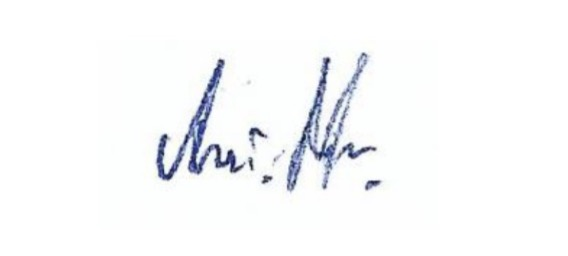
\includegraphics[width=0.8 \linewidth]{Amir_Unterschrift}}
		\caption*{Amir Al-Maytah}
	\end{center}
\end{figure}
%-----------------------------
\begin{figure}[h]
	\begin{center}
		\scalebox{0.5}
		{
\includegraphics[width=0.8 \linewidth]{Fabian_Unterschrift}}
		\caption*{Fabian Schweitzer}
	\end{center}
\end{figure}
%-----------------------------
\begin{figure}[h]
	\begin{center}
		\scalebox{0.5}
		{
\includegraphics[width=0.8 \linewidth]{Laci_Unterschrift}}
		\caption*{Ladislaus Szabo}
	\end{center}
\end{figure}
%-----------------------------

\pagebreak

%==EIDESSTATTLICHE-ERKLÄRUNG-ENDE==========================================
%==========================================================================
%==DANKSAGUNG==============================================================

\begin{center}

	\hfill \break
	\hfill \break
	\hfill \break
	\hfill \break
	\hfill \break
	\title{\textbf{\LARGE{Danksagung}}}	
	\maketitle

\end{center}

\hfill \break
\\
Wir möchten uns herzlich bei unserem Betreuer Dipl.-Ing. Christoph Diemberger bedanken, 
der uns bei diesem Projekt grundlegend unterstützt und motiviert hat. 
\hfill \break
\\
Des Weiteren gilt unser Dank auch Fachlehrer Robert Offner und allen anderen Lehrpersonen, 
die uns in der Werkstatt betreut und geholfen haben.
\hfill \break
\\
Wir danken allen, die uns im Rahmen dieses Projekts zur Seite standen.

\pagebreak

%==DANKSAGUNG-ENDE=========================================================
%==========================================================================
%==INHALT==================================================================

\tableofcontents

%--------------------------------------------------------------------------
%--------------------------------------------------------------------------

\pagebreak

\section{Einleitung}

\subsection{Kurzfassung}
\textbf{Aufgabenstellung:} 
Im Rahmen eines Diplomprojekts soll eine Roboterhand mittels eines Handschuhs gesteuert werden. 
Dazu müssen verschiedene Sensoren auf Genauigkeit getestet und aanscließend die ausgewerteten Daten kabellos an die
Roboterhand übertragen werden. Die Bewegungen der Finger sollen mit Motoren nachgebildet werden und die Stellungen
dieser soll im User-Interface dargestellt werden. \\
\textbf{Realisierung:} 
Die Bewegungen der menschlichen Hand werden mit Flexsensoren am Handschuh erfasst. Die benötigten Daten werden
anschließend über ein drahtloses Protokoll an die Roboterhand übertragen. Die Bewegungen der Roboterfinger werden mit
Servomotoren realisiert. Als User-Interface soll eine Application dienen. \\
\textbf{Ergebnis:} 
Die Handbewegungen können korrekt ausgewertet und übertragen werden. Der Benutzer trägt den Handschuh und greift 
ein Objekt. Die Servomotoren interpretieren mittels des PCBs die empfangenen Daten und ermöglichen es der Roboterhand 
ebenfalls das gleiche Objekt zu greifen. Beim Öffnen der Hand muss sich die Roboterhand in ihre Ausgangsstellung 
zurückbewegen.

\subsection{Abstract}
\textbf{Task:} 
As part of a feasibility study, a robotic hand is to be controlled by means of a glove. For
this purpose, various sensors must be tested for accuracy and the evaluated data then
transmitted wirelessly to the robotic hand. The positions of the fingers are to be displayed in a
user interface. \\
\textbf{Realization:} 
The movements of the human hand are recorded with Flex sensors on the glove.
The required data is then transmitted to the robotic hand via Bluetooth. A website will serve as
the user interface. \\
\textbf{Result:} 
The hand movements can be correctly evaluated and transmitted. The user wears the
glove and grasps an object. The servo motors interpret the received data by means of the PCB
and enable the robot hand to also grasp the same object. When the hand is opened, the robot
hand must also move back to its starting position.

\subsection{Ausgangslage}
Es gibt Produktionsbereiche, die klinisch sauber gehalten werden müssen, da durch Menschen Kontaminationen entstehen
können. Für dieses Vorhaben soll ein Prototyp einer Roboterhand, die über einen Sensorhandschuh kabellos gesteuert wird,
entwickelt und aufgebaut werden. Diverse Parameter der Roboterhand sollen in einem Interface für den Benutzer 
dargestellt werden.

\subsection{Untersuchungsanliegen der individuellen Themenstellungen}
Mit dieser Diplomarbeit soll eine Roboterhand nach einem fertigen Design aufgebaut werden,
die mit einem kabellos angebundenen Handschuh gesteuert wird. Zu diesem Zweck müssen
verschiedene Sensoren getestet werden, die die Fingergelenksstellung messen. Deren Daten
müssen ausgelesen und mittels kabelloser Schnittstelle an die Roboterhand übertragen werden
(Schweitzer). Um die Fingerbewegungen an der Roboterhand nachzustellen, muss folglich eine
Motoransteuerung entwickelt werden (Szabo). Um die elektronischen Bauelemente
unterzubringen, muss ein entsprechendes Gehäuse, in Form einer menschlichen Hand
beziehungsweise eines Arms, gefertigt werden. Zusätzlich soll ein Interface erstellt werden, in
dem der Benutzer Daten des Roboterarms und des Handschuhs einsehen kann. (Al-Maytah)

\subsection{Allgemeine Zielsetzung}
Ziel des Projekts ist es, eine Roboterhand zu bauen, die über einen kabellos verbundenen
Handschuh gesteuert werden kann. Das Ziel ist es, Daten der Fingergelenkssensoren auszulesen,
zu übertragen und die Bewegungen mit der Roboterhand nachzustellen. Endziel ist es, Daten
richtig zu verarbeiten und die Roboterhand entsprechend zu bewegen. Daten sollen in einem
Interface dargestellt werden.

\subsection{Terminplan (Milestones)}
Lastenheft fertig – 10.10.2023 \\
Kostenkalkulationen fertig – 24.10.2023 \\
Prototypen proof of concept –21.11.2023 \\
Hardwaredesign fertig – 05.12.2023 \\
PCB-Design fertig – 09.01.2024 \\
Softwareimplementierung für Integrationstest fertig - 30.01.2024 \\
Integration aller Komponenten – 06.02.2024 \\
User Interface fertiggestellt – 13.02.2024 \\
Abnahme durch die Projektbetreuer – 12.03.2024

\subsection{Geplantes Ergebnis der Prüfungskandidaten}
Es soll eine Erfassung der Sensordaten möglich sein. Diese sollen übertragen und empfangen
werden können. Die Roboterhand soll die Finger nach der Vorgabe des Handschuhs bewegen
können. Als Endergebnis soll eine halbvolle 500mL Plastikflasche umschlossen und in der Luft
gehalten werden. In dem Interface, dem User-Interface, sollen wichtige Daten dargestellt und
Parameter verändert werden können.

\subsection{Entwicklungsteam}
Folgende Schüler des TGMs haben sich mit der Entwicklung des in Punkt 1.1 beschrieben Projekts befasst: \hfill \break
\\
Projektleiter:    Ladislaus Szabo (Hardwareentwicklung, PCB-Design, Projektleitung)\\
Mitarbeiter: Fabian Schweitzer (Mikrokontroller-Programmierung, Testmanagement, Gesamtintegration)\\
Amir Al-Maytah (3D-Druck, Mechanik, Userinterface-Programmierung)

\hfill \break
\hfill \break
\hfill \break
\hfill \break
\hfill \break
\hfill \break
\hfill \break
\hfill \break

%--------------------------------------------------------------------------
%--------------------------------------------------------------------------

\section{Anforderungen der einzelnen Projektteile}

\subsection{Mechanik}
\subsubsection{Handschuh}
Folgende machanische Anforderungen muss der Handschuh nach Abschluss des Projekts erfüllen:

\subsubsection{Roboterhand}
Folgende mechanische Anforderungen muss der Handschuh nach Abschluss des Projekts erfüllen:

	\begin{itemize}
		\item Die Roboterhand/der Roboterarm soll mittels 3D-Druck gefertigt werden.
		\item Die Servomotoren der Elektronik werden mithilfe von Schnüren mit den jeweiligen Fingern verbunden.
		\item Die Finger sollen sich sowohl zum Handballen als auch vom Handballen weg kontrolliert bewegen können.
		\item Die Finger sollen sich zitterfrei bewegen können.
	\end{itemize}

\subsection{Eletronische Hardware}
\subsection{Handschuh}
Folgende elektronische Anforderungen muss der Handschuh nach Abschluss des Projekts erfüllen:

\subsubsection{Roboterhand}
Folgende elektronische Anforderungen muss die Roboterhand nach Abschluss des Projekts erfüllen:

	\begin{itemize}
		\item Die Bewegung der Finger muss mit Sensoren erfasst werden.
		\item Die Sensordaten müssen mit einem Mikrokontroller ausgewertet werden können.
		\item Der zur Datenerfassung gewählte Mikrokontroller muss:
		\begin{itemize}
			\item Die I2C Kommunikation unterstützen.
			\item Die Möglichkeit für eine kabellose Kommunikation aufweisen.
			\item Analoge und Digitale Eingänge haben.
			\item Programmierbar sein.
		\end{itemize}
		\item Es muss möglich sein, mindestens 30 verschiedene Sensorwerte, von minimaler bis maximaler Fingerbeugung, 
		      zu erfassen.
		\item Der RoboGlove muss die Möglichkeit zur Versorgung mit einem Akku oder einer Batterie und einem Netzteil 
		      aufweisen. 
		\item Jeder Finger der „Bionic Hand“ soll durch einen eigenen Motor gesteuert werden.
		\item Jeder dieser Motoren muss individuell regelbar sein, um die Griffkraft der Hand zu kontrollieren.	
		\item Jeder Finger soll sich zum Handballen beugen und wieder strecken lassen.	
		\item Diese Bewegungen sollen störungsfrei und ohne zittern erfolgen.
	\end{itemize}

\subsection{Software}
\subsubsection{Handschuh}
Folgende Software Anforderungen muss der Handschuh nach Abschluss des Projekts erfüllen:

\subsubsection{Roboterhand}
Folgende Software Anforderungen muss der Handschuh nach Abschluss des Projekts erfüllen:

	\begin{itemize}
		\item Der Widerstand jedes Flexsensors, der an jedem Handschuh jeweils über jedem Finger angebracht ist, 
			  soll einzeln ausgelesen werden können. Die Software soll damit feststellen, wie sehr der Flexsensor 
			  gebogen ist.
		\item Diese Daten sollen erfolgreich eingelesen werden und direkt an die Empfängerplatine gesendet werden.
	\end{itemize}

\subsubsection{Bionische Hand}
Folgende Anforderungen müssen für die Software für die Roboterhandplatine nach Abschluss des Projekts erfüllt sein:

	\begin{itemize}
		\item Die von der Handschuhplatine gesendeten Daten sollen erfolgreich empfangen und gespeichert werden.
		\item Eine Fehlerkorrektur sorgt dafür, dass die empfangenen Daten richtig verarbeitet werden können.
		\item Die Software muss bei jedem Finger etwas anders agieren, da die Widerstandswerte der verschiedenen 
		      Flexsensoren .
			  stark variieren. Es soll bei jedem Finger eine gleich gute Steuerung der Roboterhand möglich sein.
		\item Es muss immer wieder (alle 10ms) der Strom gemessen werden. Mit einem Timing Interrupt muss also zwischen 
		      dem Bewegen der Finger immer wieder dieser gemessen werden.
		\item Es sollen unterschiedliche Modi erstellt werden, je nachdem, was mit der Roboterhand gehalten werden soll. 
			  Die Griffkraft soll je nach Objekt variieren.
	\end{itemize}

\subsubsection{User Interface}

%--------------------------------------------------------------------------
%--------------------------------------------------------------------------

\section{Detailierte Beschreibung der Projektteile}

\subsection{Handschuh (Eingabe)}
Der Handschuh ermöglicht dem Benutzer die Roboterhand zu steuern. 
Dies geschieht durch Flexsensoren, die an den Fingern des Handschuhs angebracht sind. Wird ein Finger gebeugt, 
so ändert sich der Widerstand des Sensors. Diese Änderungen werden von einem Mikrokontroller erfasst, ausgewertet 
und für die kabellose Übertragung an die Roboterhand vorbereitet. Damit dem Handschuh funktioniert, bedarf es 
einer Spannungsversorgung. Diese wird in Form einer Batterie oder eines Akkus vorgesehen sein. Für einen möglichen 
stationären Betrieb kann der Handschuh auch mit einem Netzteil betrieben werden. Die Passform des Handschuhs soll 
möglichst komfortabel sein, um eine möglichst lange Benützung zu ermöglichen. Dies setzt eine gut überlegte Integration 
der Elektronik voraus, die bei diesem Projekt auch bestmöglich beachtet wurde. Der Handschuh ist so gebaut, dass er 
auch von Personen ohne elektronische Ausbildung und ohne Vorwissen bedient werden kann.\\
\\
\textcolor{red}{Folgende Richtlinien und Normen werden vom Handschuh erfüllt:}\\
\\
Die Software des Roboterhandschuhs ist dafür verantwortlich die sich verändernden Widerstandswerte der Flexsensoren 
jeweils einzeln einzulesen. Über die UART-Schnittstelle wird die Software auf den ESP32 hochgeladen. Dabei werden 
direkt aus dem in der Schaltung verbauten ADC-Werte, über die I2C-Schnittstelle, ausgelesen. Man erhält bereits digitale 
Werte, die der ESP32 dann direkt in einer festgelegten Reihenfolge an die Empfängerplatine, bei der Roboterhand, per 
ESP-NOW Übertragung senden kann.

\subsection{Roboterhand (Ausgabe)}
Die Roboterhand ist die Ausgabe des Projekts und wird vom Roboterarm gesteuert. Jeder Finge wird von einem Servomotor 
bewegt. Dieser ist durch zwei dünne Schnüre mit dem korrespondierenden Finger verbunden. Die vom Handschuh kommenden 
Daten werden von einem Mikrokontroller ausgewertet und in ein PWM-Signal (Pulsweitenmodulation) zur Ansteuerung der 
Servomotoren umgewandelt. Jeder Finger hat drei Gelenke und kann daher kontrolliert gebeugt und wieder gestreckt werden. 
Die komplette Roboterhand wird mittels 3D-Druck gefertigt. Silikonprofile auf den Fingern versichern das Objekte nicht 
mehr aus dem Griff der Hand rutschen können.\\
\\
\textcolor{red}{Folgende Richtlinien und Normen werden von der Roboterhand erfüllt:}\\
\\
Die Software des Roboterarmes ist dafür verantwortlich, dass die von der Handschuhplatine, via ESP32, gesendeten Daten 
erfolgreich empfangen und gespeichert werden. Die Software wird hierzu per UART-Schnittstelle auf den ESP32 hochgeladen. 
Die Daten der Flexsensoren, die man bereits erhalten hat, sollen dann verarbeitet werden. Anhand des Widerstandwertes und 
der jeweiligen Veränderung, wird dann der Winkel des Servos eingestellt. Eine Fehlerkorrektur soll sicherstellen, dass die 
Griffkraft passend eingestellt wird. Jeder Flexsensor hat unterschiedliche Widerstandswerte, es muss also über jeden Finger 
eine gezielte Software geschrieben werden, damit man schlussendlich durch das Zusammenspiel aller Finger die Griffkraft 
richtig einstellen kann. Falsche Messungen sollen bestmöglich korrigiert werden, sodass die Servos jeweils die richtigen 
Winkeleinstellungen erhalten. Der ESP32 stellt hierbei die Zentrale der Steuerung dar.

\subsection{User Interface}

%--------------------------------------------------------------------------
%--------------------------------------------------------------------------

\section{Mechanische Entwicklung}

\subsection{Handschuh}

\subsection{Roboterhand}

%--------------------------------------------------------------------------
%--------------------------------------------------------------------------

\section{Hardwareentwicklung}

\subsection{Handschuh}

\subsubsection{Simulationen und Versuchsaufbauten}
Sensorik:
\\
Es muss in irgendeiner Weise die Fingerbeugung, beziehungsweise Bewegung, des Benutzers mit dem „RoboGlove“ gemessen 
werden können. Dies könnte man durch das Messen des Beugungswinkels realisieren. Allerdings hat jeder Finger drei Gelenke, 
wodurch man diese auch bei der „Bionic Hand“ individuell steuern müsste. Die zweite Möglichkeit wäre, durch eine visuelle 
Aufnahme die Bewegung des „RoboGlove“ und dadurch des Benutzers aufzuzeichnen. Da dies allerdings nur in dafür vorgesehenen, 
mit Kameras ausgestatteten, Räumen funktionieren würde, ist dies für uns auch keine sinnvolle Möglichkeit. Schließlich haben 
wir uns für die Erfassung der Fingerbewegungen mittels Flexsensoren entschieden. Diese ändern den Widerstand je nach der 
aktuell vorherrschenden Beugung. Bei dieser Art der Bewegungserfassung muss man nicht jedes Fingergelenk einzeln steuern und 
braucht auch keine externen Kameras. Somit ist bei dieser Methode der Datenerfassung ein sehr flexibler Verwendungsbereich 
des „RoboGlove“ gewährleistet.\\
\\
Auslesen der Sensoren:
\\
Das Auslesen der Flexsensoren kann durch einen einfachen Spannungsteiler erfolgen. Dabei ist die Genauigkeit (Auflösung) 
allerdings nicht gegeben und ist daher nicht für unsere Anwendung geeignet. Die Lösung für dieses Genauigkeitsproblem ist 
eine ADC-Schaltung mit einer davor geschalteten OPV-Schaltung.

\begin{figure}[h]
	\begin{center}
	\scalebox{0.5}
	{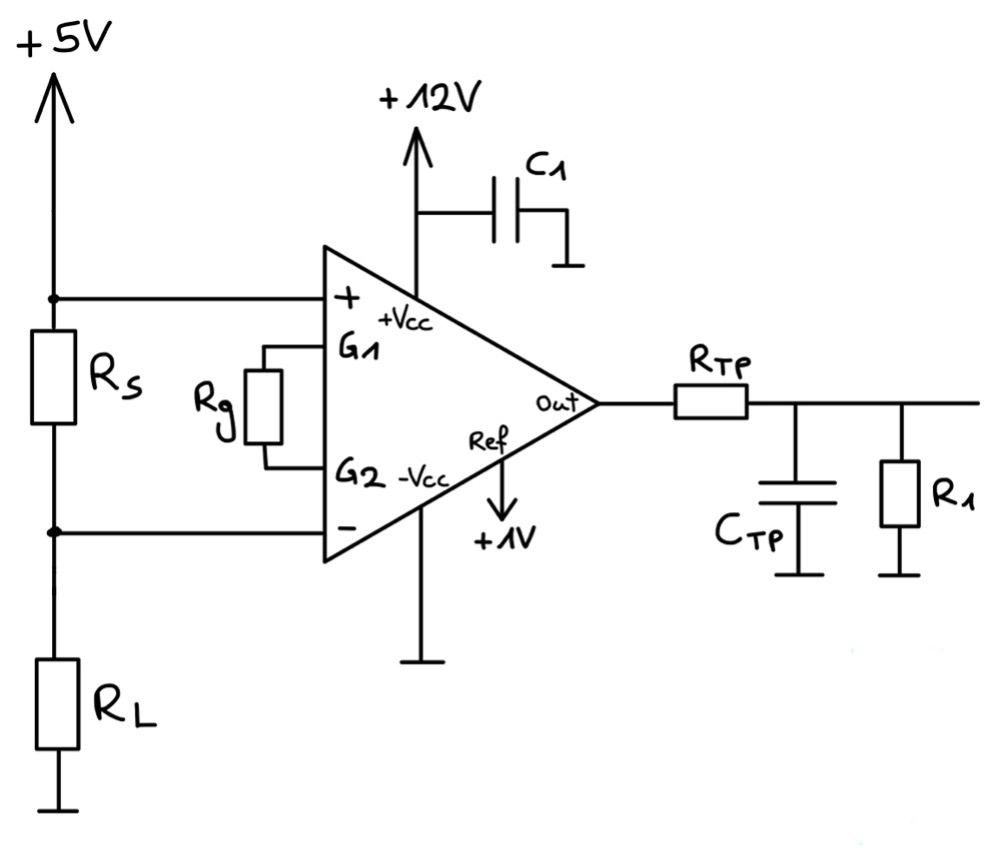
\includegraphics[width=0.8 \linewidth]{Messschaltung_Handschuh_Spannung}}
	\caption{Messchaltung Spannungsmessung}
	%\label{fig:schaltung3}
	\end{center}
\end{figure}

Der Flexsensor (RL) bezieht seine Versorgung über einen Shunt-Widerstand (Rs). Je nach Belastung, ändert sich der 
Spannungsabfall an diesem (Je größer die Beugung des Sensors, desto kleiner ist der Spannungsabfall). Die Spannungsdifferenz 
am Shunt-Widerstand wird von einem Operationsverstärker verstärkt. Ein Tiefpassfilter (Rtp und Ctp) ist hinter den Ausgang des 
OPV geschaltet, um mögliche Spannungsstörungen (Ripple) herauszufiltern. Der zu GND geschaltete Widerstand (R1), entlastet 
den Eingang des angeschlossenen ADCs. Dieser Analog-Digital-Wandler digitalisiert das analoge Eingangssignal und überträgt 
diese an den verbauten Mikrokontroller. Da die OPV-Messschaltung verhältnismäßig viel Platz in Anspruch nimmt und diese 
fünfmal, für jeden Flexsensor einmal, benötigt wird, wäre es von großem Vorteil alle Sensoren mit nur einer Schaltung 
auszumessen. Hierfür verwenden wir einen Multiplexer, der in Bruchteilen einer Sekunde zwischen allen Biegemessstreifen 
durchschaltet. Dies ermöglicht das Auslesen aller Sensoren mit nur einer Verstärkerschaltung und trägt wesentlich zur 
möglichst kompakten Dimensionierung der später folgenden Platine bei.\\
\\
Mikrokontroller:
\\
Der zur Auswertung der Messdaten zuständige Mikrokontroller muss, die in Punkt 2.2.1 angeführten Anforderungen, erfüllen. 
Hierzu haben wir uns für den ESP32 entschieden, da dieser mehr als genug Rechenleistung bietet, mehrere drahtlose 
Übertragungsmöglichkeiten unterstützt und die Möglichkeit einer Verbindung mit dem Internet bietet. Der kleine Formfaktor, 
trotz den vielen IO-Ports, ist nur ein weiteres Argument für die Wahl dieses Mikrokontrollers. Um den ESP32 programmieren 
und steuern zu können, sind zwei Taster, einer für das RESET und einer für den UPLOAD, notwendig. Außerdem ist ein 
Mikro-USB-Anschluss notwendig, um den in einer Entwicklungsumgebung erstellten Code hochzuladen. Da man die USB-Buchse 
nicht direkt mit dem ESP32 verbinden kann, ist zusätzlich noch ein Bustreiber notwendig, der ein am Mikrokontroller 
vorhandenes Interface unterstützt.  

\subsubsection{Überlegungen und Berechnungen}

\textcolor{red}{Bild der Spannungs-Simulation hier einfügen!!}\\
\\
Der Widerstand der Flexsensoren ändert sich bei zunehmender Beugung von 25k\textOmega auf 125k\textOmega.\\
\\
\textcolor{red}{Hier das Messprotokoll der Flexsensoren einfügen!!}\\
\\
Die Flexsensoren werden mit +5V Gleichspannung versorgt. Zwischen der Versorgung und den Sensoren ist ein Shunt-Widerstand 
(RS) geschaltet, an dem je nach Beugung der Sensoren eine gewisse Spannung abfällt. Dies ist der Fall, da bei einem 
geringeren Widerstand des Flexsensors ein größerer Strom über den Widerstand RS fließt und somit der Spannungsabfall größer 
ist. Bei großen (niederohmigen) Lasten ist es sehr wichtig dabei die Verlustleistung am Shunt zu beachten, allerdings ist 
dies bei Flexsensoren kein Thema, da diese nur einen sehr kleinen Strom benötigen.
\\
Um nun die korrekte Verstärkung des OPVs und den korrekten Shunt-Widerstand zu wählen ist es wichtig zu wissen, dass wir 
einen 10-Bit ADC mit +3.3V Versorgungsspannung verwenden. Mit dieser Information haben wir nun den Shunt und den Widerstand 
Rg dimensioniert. Die Ausgangsspannung des Verstärkers bei maximaler Last des Flexsensors sollte knapp unter +3.3V sein, 
um die Auflösung des ADCs maximal auszunützen. Zuerst haben wir die Verstärkung G=78 gewählt, da bei einem höheren Gain 
Störungen auftreten könnten. Dafür wurde aus dem Datenblatt des OPVs der Widerstand Rg mit 1.1kOhm gewählt. Mit dieser 
Information haben wir dann den Shunt Rs mit 240OHM dimensioniert. Da bei größeren Widerständen des Flexsensors der 
Spanungsabfall allerdings so gering ist, dass der Operationsverstärker diesen nicht mehr exakt verstärken kann, ist es 
notwendig eine +1V Referenzspannung am OPV anzulegen. Durch diese kann auch bei sehr kleinen Spannungsabfällen ein exakt 
verstärktes Ausgangssignal generiert werden.\\
\\
\textcolor{red}{Dimensionierung Spannungsteiler für +1V hier einfügen!!}\\
\\
Durch den Tiefpass am Ausgang werden mögliche Spannungsripple der Versorgung gefiltert. Durch den Widerstand Rtp wird 
ein kleiner Spannungsabfall erzeugt, der bei der Messung zwar berücksichtigt wird, allerdings kein Problem darstellt. 
Die Grenzfrequenz des Filters wurde folgender Maßen berechnet:\\
\\
\textcolor{red}{Berechnung fg hier einfügen!!}\\
\\
Durch den zu GND geschalteten Widerstand R1 mit 10kOHM, wird er Eingang des danach kommenden ADCs entlastet. 

\subsubsection{Schaltplandesign}
\subsubsection{Platinendesign}

\subsection{Roboterhand}
\subsubsection{Simulationen und Versuchsaufbauten}
\subsubsection{Überlegungen und Dimensionierung}
\subsubsection{Schaltplandesign}
\subsubsection{Platinendesign}

%--------------------------------------------------------------------------
%--------------------------------------------------------------------------

\section{Softwareentwicklung}

\subsection{Handschuh}
\subsubsection{Konzepte und Überlegungen}
\subsubsection{Realisierung und Gliederung}

\subsection{Roboterhand}
\subsubsection{Konzepte und Überlegungen}
\subsubsection{Realisierung und Gliederung}

\subsection{User Interface}
\subsubsection{Entwicklungsumgebung}
\subsubsection{Konzepte und Überlegungen}
\subsubsection{Realisierung und Gliederung}

%--------------------------------------------------------------------------
%--------------------------------------------------------------------------

\section{Abschluss und Zusammenfassung}

%--------------------------------------------------------------------------
%--------------------------------------------------------------------------

\section{Anhang}
\section{Quellen -und Literaturverzeichnis}
\section{Abbildungsverzeichnis}

\end{document}